\appendix

\begin{figure}[H]
	\centering
	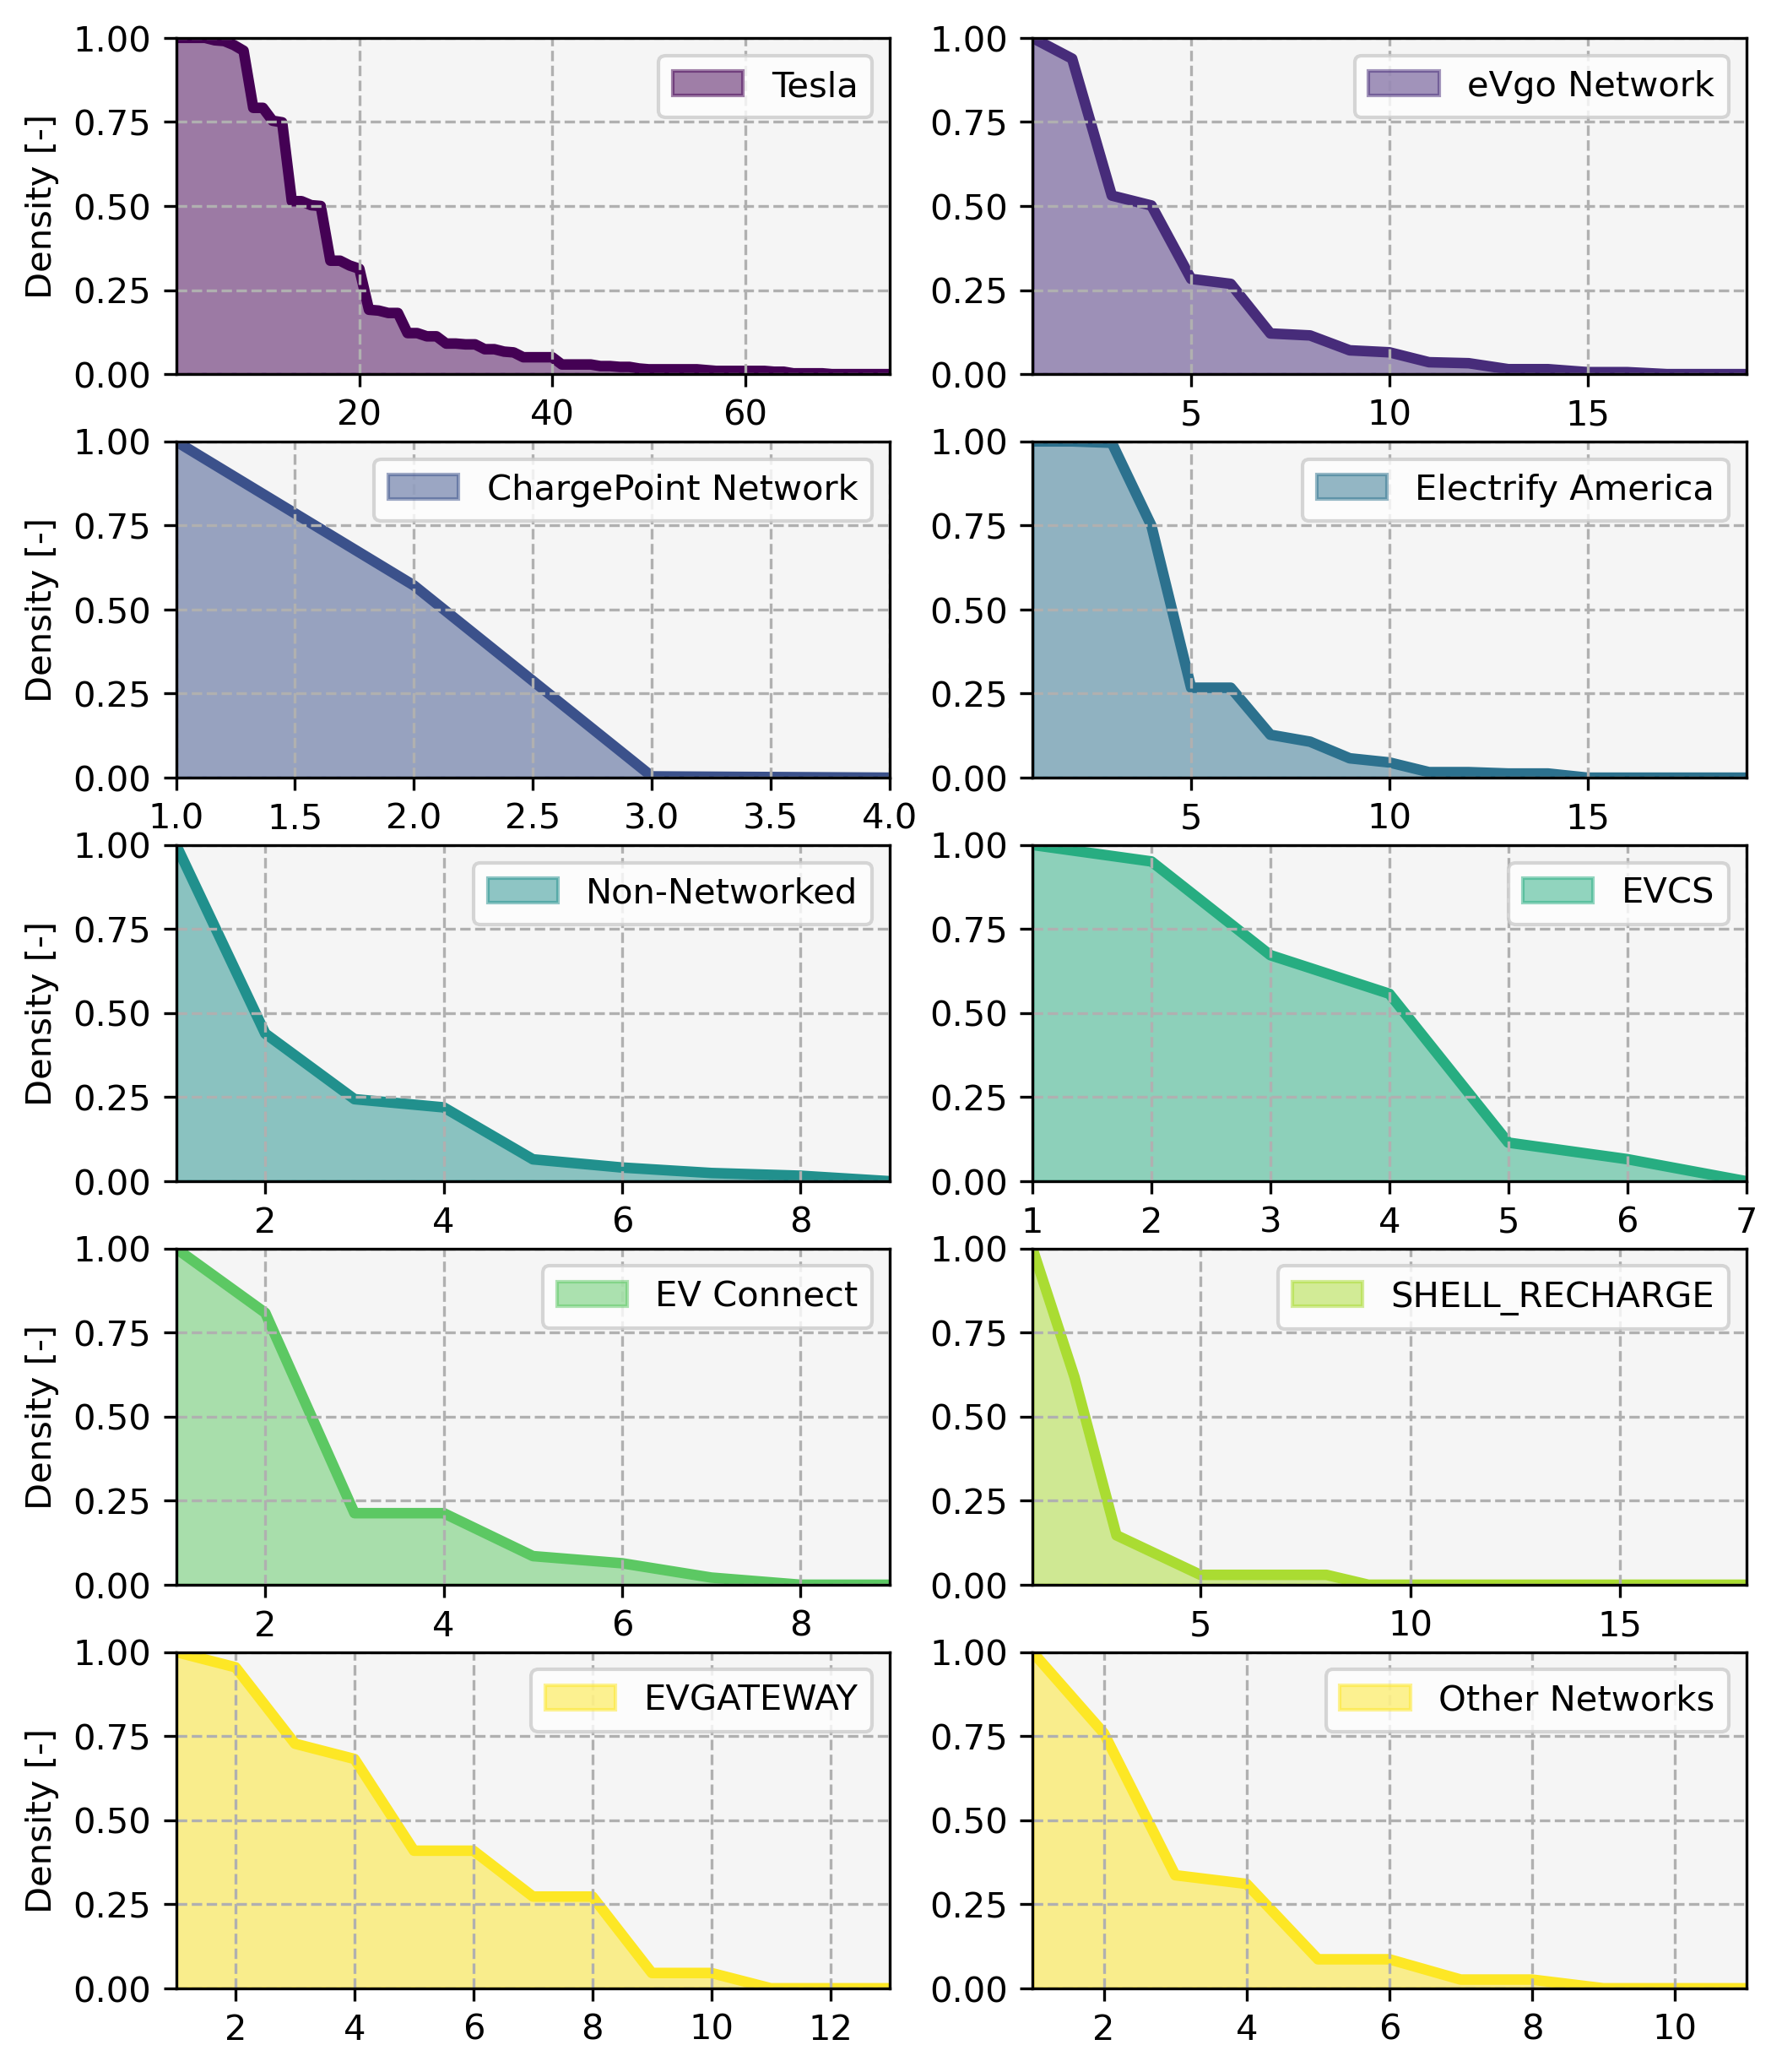
\includegraphics[width = \linewidth]{figs/California_RIS_SF_All.png}
	\caption{In-station redundancy for DC Charging networks in California}
	\label{fig:ris_top_networks}
\end{figure}

\begin{figure}[H]
	\centering
	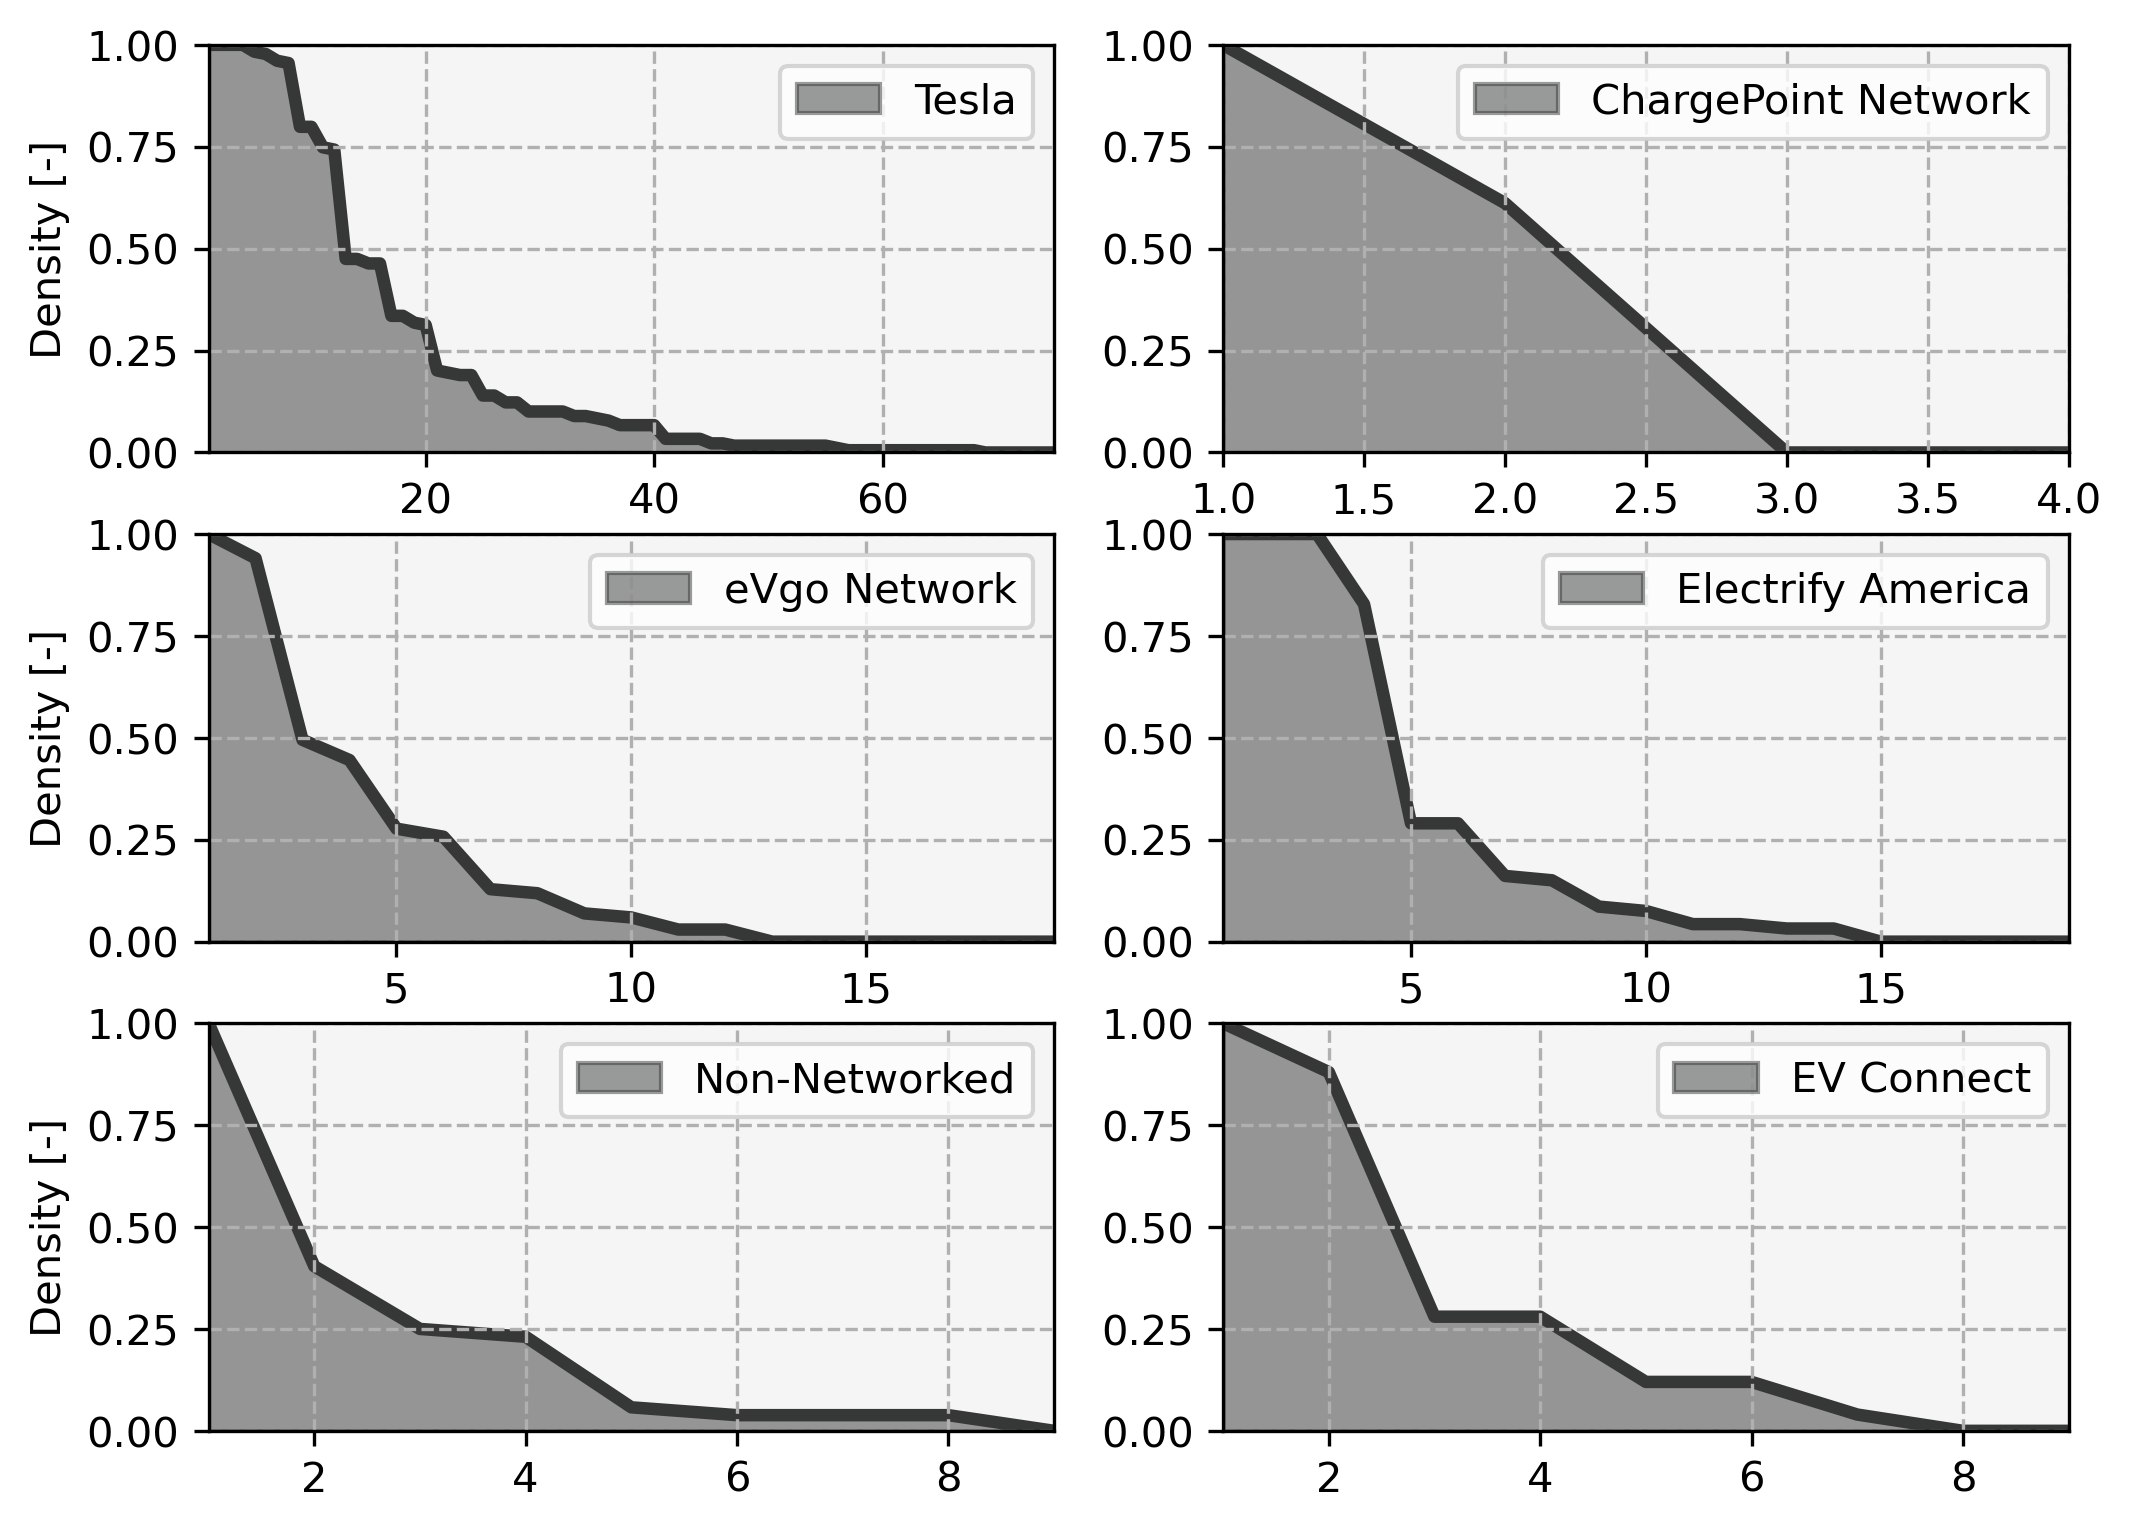
\includegraphics[width = \linewidth]{figs/California_RIS_SF_Corridor.png}
	\caption{In-station redundancy for DC Charging networks in California}
	\label{fig:ris_top_networks_corridor}
\end{figure}


%\begin{figure}[H]
%	\centering
%	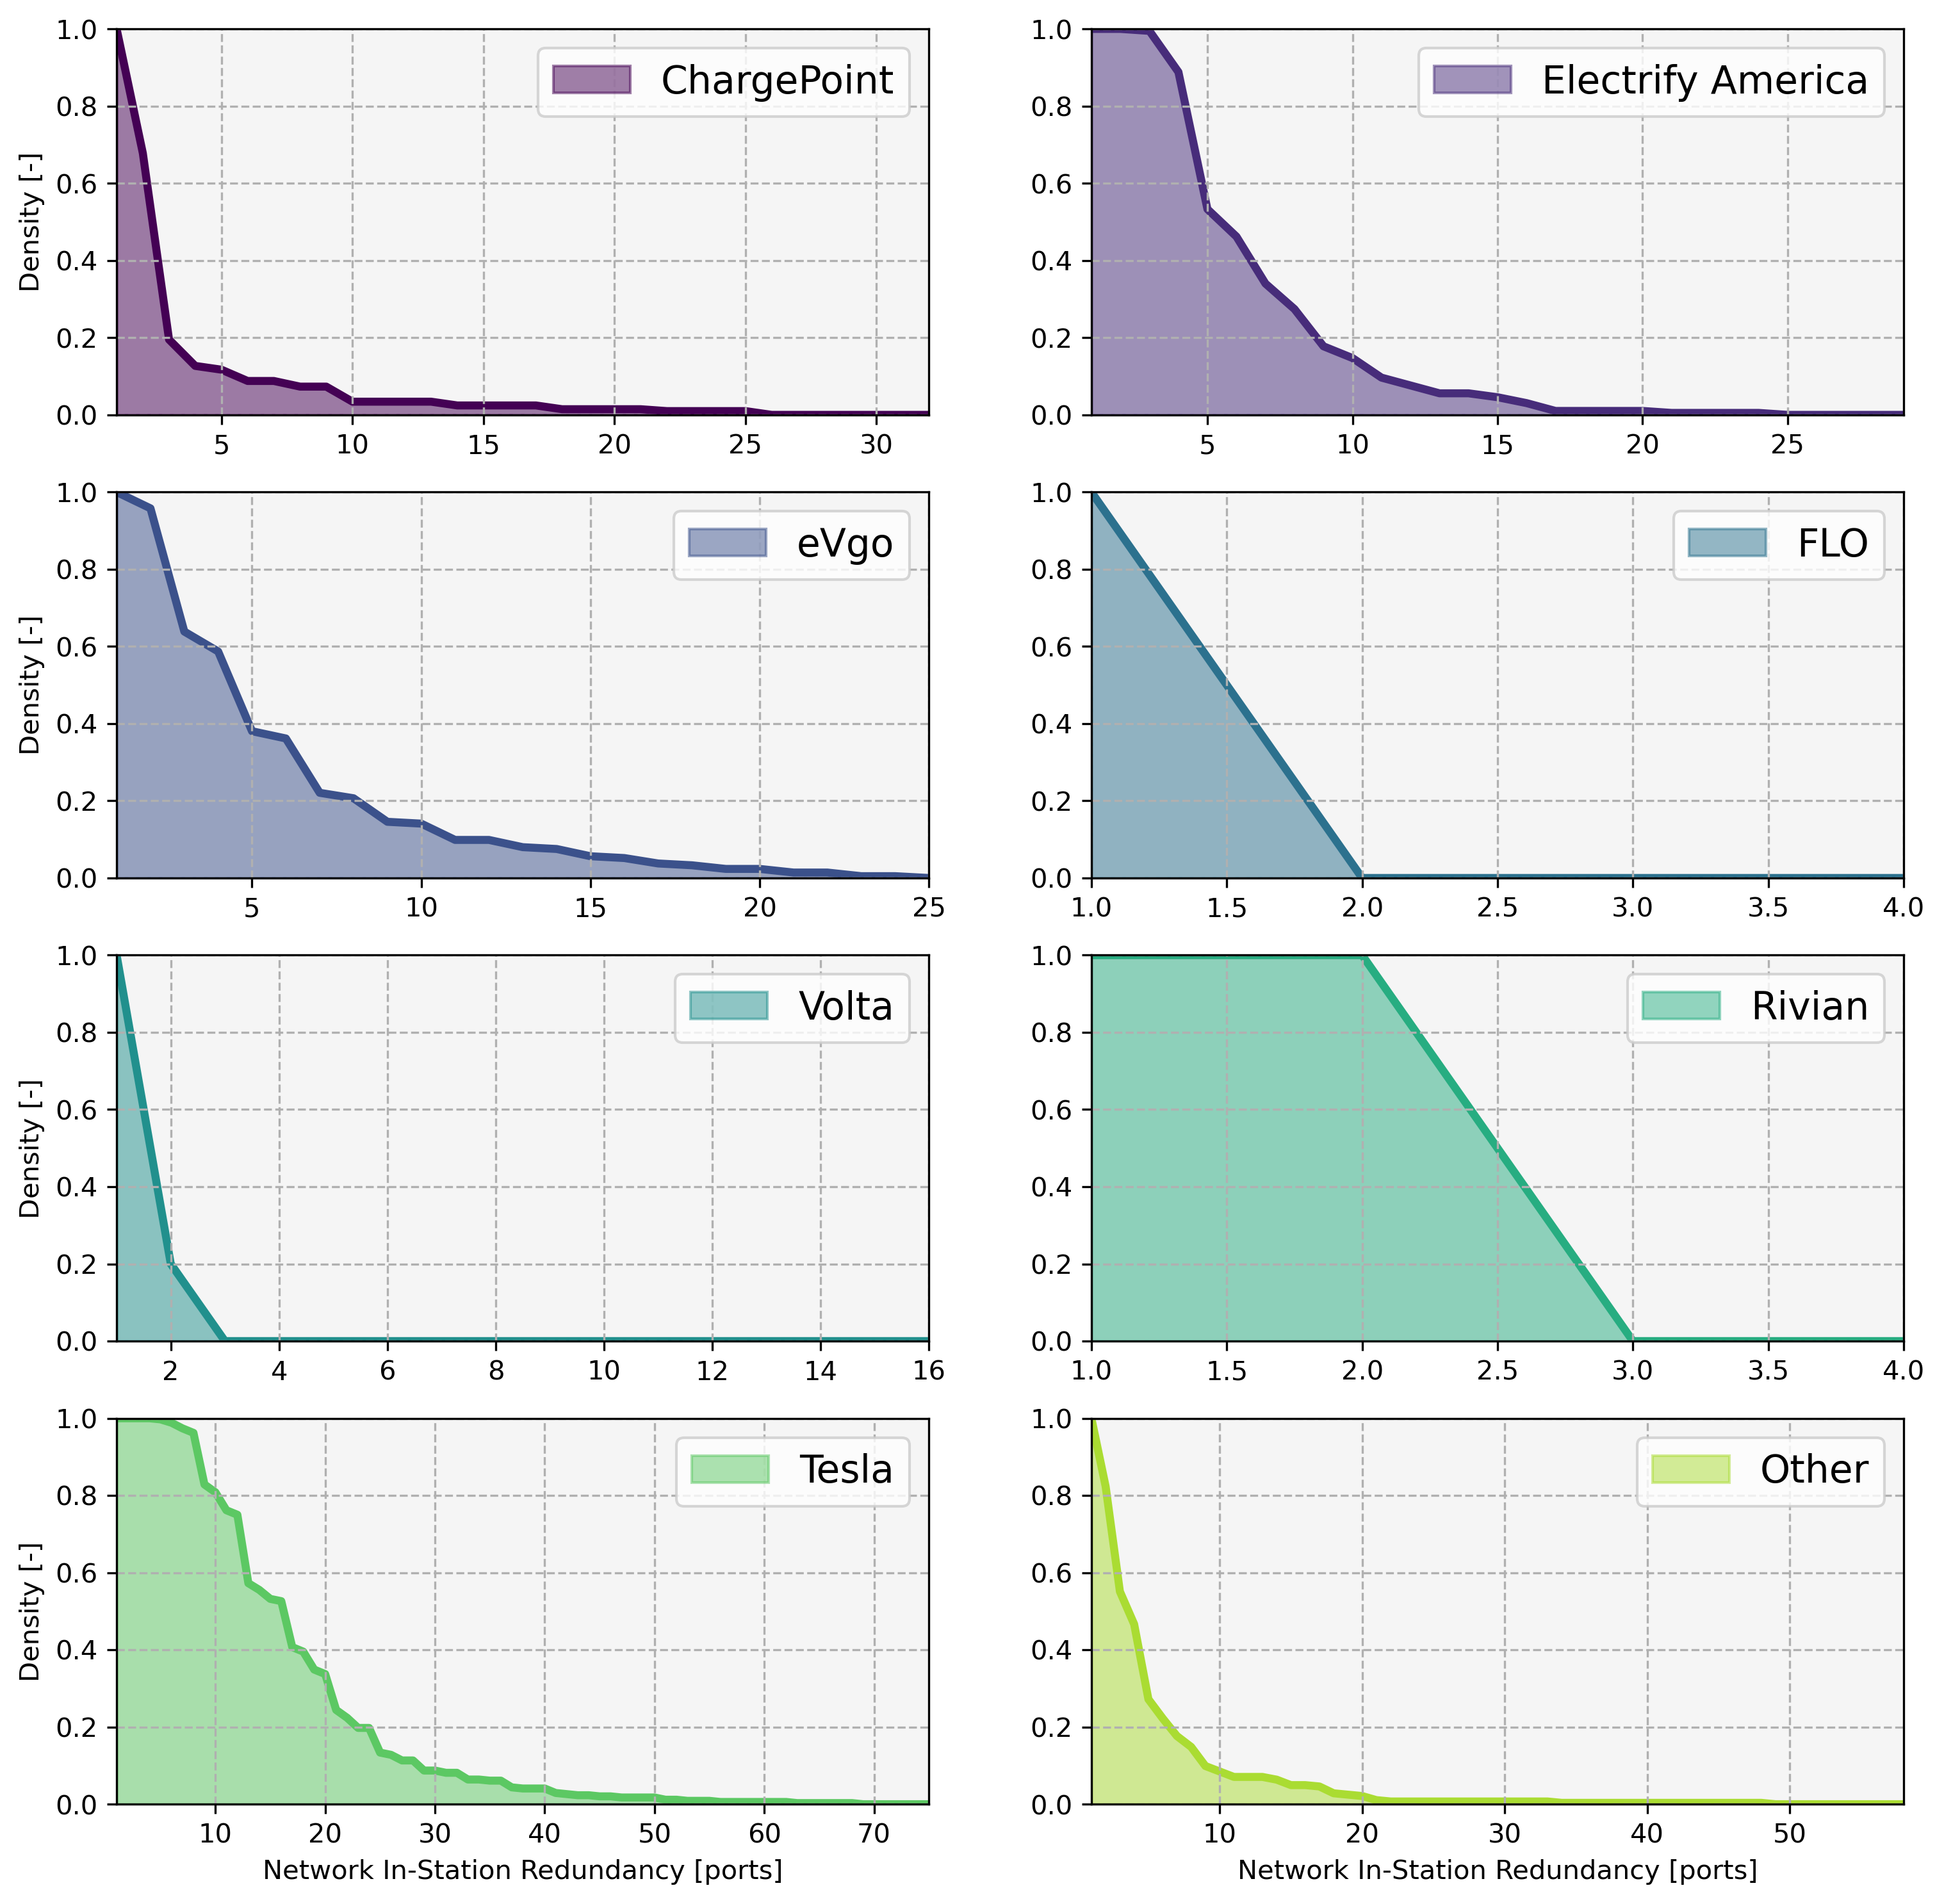
\includegraphics[width = \linewidth]{figs/California_RBS_300_SF_All.png}
%	\caption{In-station redundancy for DC Charging networks in California}
%	\label{fig:rbs_300_top_8_networks}
%\end{figure}
%
%
%\begin{figure}[H]
%	\centering
%	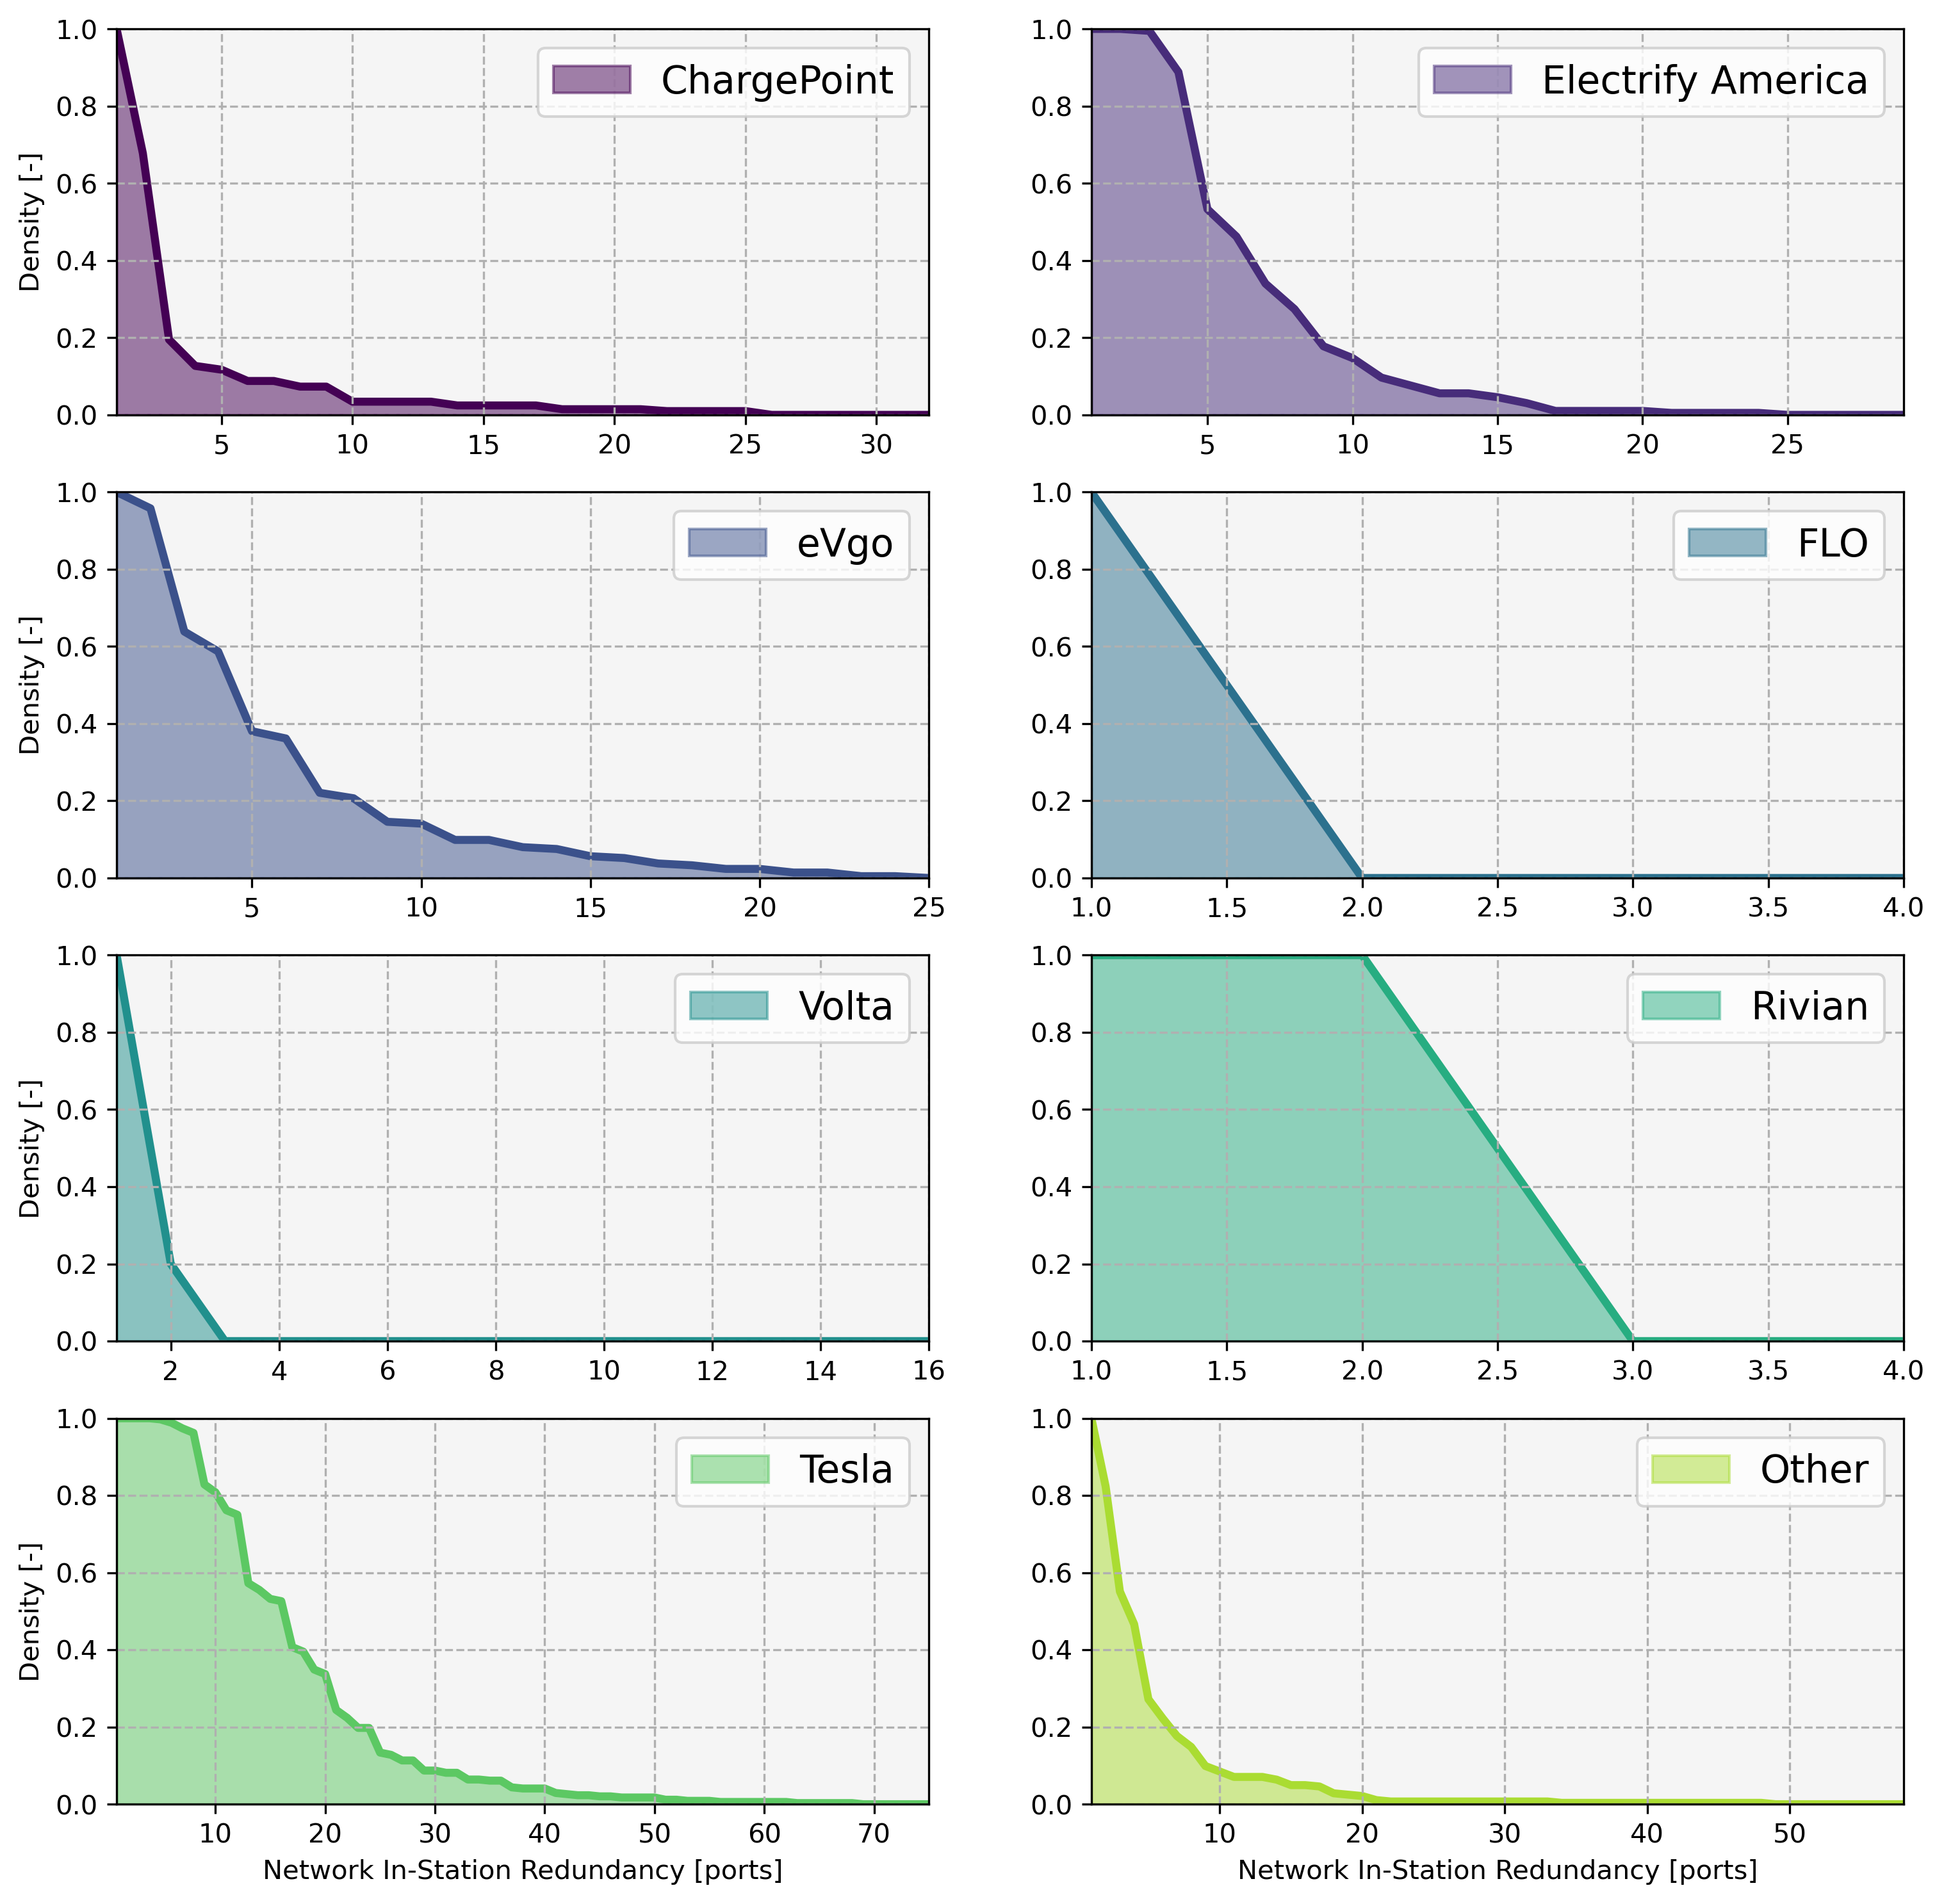
\includegraphics[width = \linewidth]{figs/California_RBS_600_SF_All.png}
%	\caption{In-station redundancy for DC Charging networks in California}
%	\label{fig:rbs_600_top_8_networks}
%\end{figure}

\begin{table}[H]
	\centering
	\caption{Summary statistics for California DC charging networks from \gls{afdc}}
	\label{tab:summary_statistics_afdc}
	\begin{tabular}{|C{.46\linewidth}|C{.18\linewidth}|C{.18\linewidth}|C{.18\linewidth}|}
		\hline Network & Chargers & Stations & Chargers per Station \\
		\hline Non-Networked & 288 & 51 & 5.6 \\
		\hline Tesla & 2753 & 156 & 17.6 \\
		\hline Electrify America & 526 & 77 & 6.8 \\
		\hline EV Connect & 59 & 19 & 3.1 \\
		\hline ChargePoint Network & 186 & 79 & 2.4 \\
		\hline Volta & 2 & 2 & 1.0 \\
		\hline EVCS & 41 & 11 & 3.7 \\
		\hline SHELL_RECHARGE & 39 & 11 & 3.5 \\
		\hline EVGATEWAY & 21 & 5 & 4.2 \\
		\hline eVgo Network & 332 & 63 & 5.3 \\
		\hline BP_PULSE & 3 & 2 & 1.5 \\
		\hline POWERFLEX & 12 & 3 & 4.0 \\
		\hline FLO & 1 & 1 & 1.0 \\
		\hline EVRANGE & 11 & 3 & 3.7 \\
		\hline RIVIAN_ADVENTURE & 14 & 7 & 2.0 \\
		\hline CIRCLE_K & 16 & 3 & 5.3 \\
		\hline CHARGENET & 7 & 1 & 7.0 \\
		\hline Blink Network & 2 & 2 & 1.0 \\
		\hline NOODOE & 2 & 1 & 2.0 \\
		\hline LOOP & 6 & 2 & 3.0 \\
		\hline 7CHARGE & 4 & 1 & 4.0 \\
		\hline
	\end{tabular}
\end{table}

\begin{table}[H]
	\centering
	\caption{Summary statistics for California DC charging networks from \gls{afdc} (corridor stations)}
	\label{tab:summary_statistics_afdc_corridor}
	\begin{tabular}{|C{.46\linewidth}|C{.18\linewidth}|C{.18\linewidth}|C{.18\linewidth}|}
		\hline Network & Chargers & Stations & Chargers per Station \\
		\hline Non-Networked & 274 & 50 & 5.5 \\
		\hline Tesla & 2745 & 155 & 17.7 \\
		\hline Electrify America & 518 & 76 & 6.8 \\
		\hline EV Connect & 58 & 18 & 3.2 \\
		\hline ChargePoint Network & 184 & 78 & 2.4 \\
		\hline Volta & 1 & 1 & 1.0 \\
		\hline EVCS & 35 & 10 & 3.5 \\
		\hline SHELL_RECHARGE & 37 & 10 & 3.7 \\
		\hline EVGATEWAY & 19 & 4 & 4.8 \\
		\hline eVgo Network & 329 & 62 & 5.3 \\
		\hline BP_PULSE & 1 & 1 & 1.0 \\
		\hline POWERFLEX & 10 & 2 & 5.0 \\
		\hline EVRANGE & 5 & 2 & 2.5 \\
		\hline RIVIAN_ADVENTURE & 12 & 6 & 2.0 \\
		\hline CIRCLE_K & 12 & 2 & 6.0 \\
		\hline Blink Network & 1 & 1 & 1.0 \\
		\hline LOOP & 2 & 1 & 2.0 \\
		\hline
	\end{tabular}
\end{table}

\begin{table}[H]
	\centering
	\caption{Linear Regression Analysis ANOVA}
	\label{tab:regression_anova}
	\begin{tabular}{|C{.25\linewidth}|C{.25\linewidth}|C{.25\linewidth}|C{.25\linewidth}|}
		\hline R & R-Squared & Adjusted R-Squared & Std. Error \\
		\hline 0.930 & 0.865 & 0.860 & 0.000 \\
		\hline
		\hline Category & Sum of Squares & DOF & Mean Squares \\
		\hline Model & 405.979 & 47 & 8.638 \\
		\hline Error & 63.621 & 1452 & 0.044 \\
		\hline Total & 469.601 & 1499 & 0.313 \\
		\hline  \multicolumn{2}{|c|}{$F$} &  \multicolumn{2}{c|}{$P(>F)$}  \\
		\hline  \multicolumn{2}{|c|}{197.138} &  \multicolumn{2}{c|}{0.000}  \\
		\hline
	\end{tabular}
\end{table}

\begin{table}[H]
	\centering
	\caption{Linear Regression Analysis Coefficients and P-Values}
	\label{tab:regression_coefficients}
	\begin{tabular}{|C{.5\linewidth}|C{.25\linewidth}|C{.25\linewidth}|}
		\hline Parameter & Coefficient & P-Value \\
		\hline {\small Intercept } & 5.245 & 0.000 \\
		\hline {\small capacity } & -1.417 & 0.000 \\
		\hline {\small Tesla Only } & 0.037 & 0.005 \\
		\hline {\small charge_rate } & -0.273 & 0.000 \\
		\hline {\small reliability } & -0.504 & 0.000 \\
		\hline {\small arrival_ratio } & 0.701 & 0.000 \\
		\hline {\small risk_attitude } & 0.669 & 0.000 \\
		\hline {\small Non-Tesla Only } & 0.102 & 0.000 \\
		\hline
	\end{tabular}
\end{table}

%\begin{figure}[H]
%	\centering
%	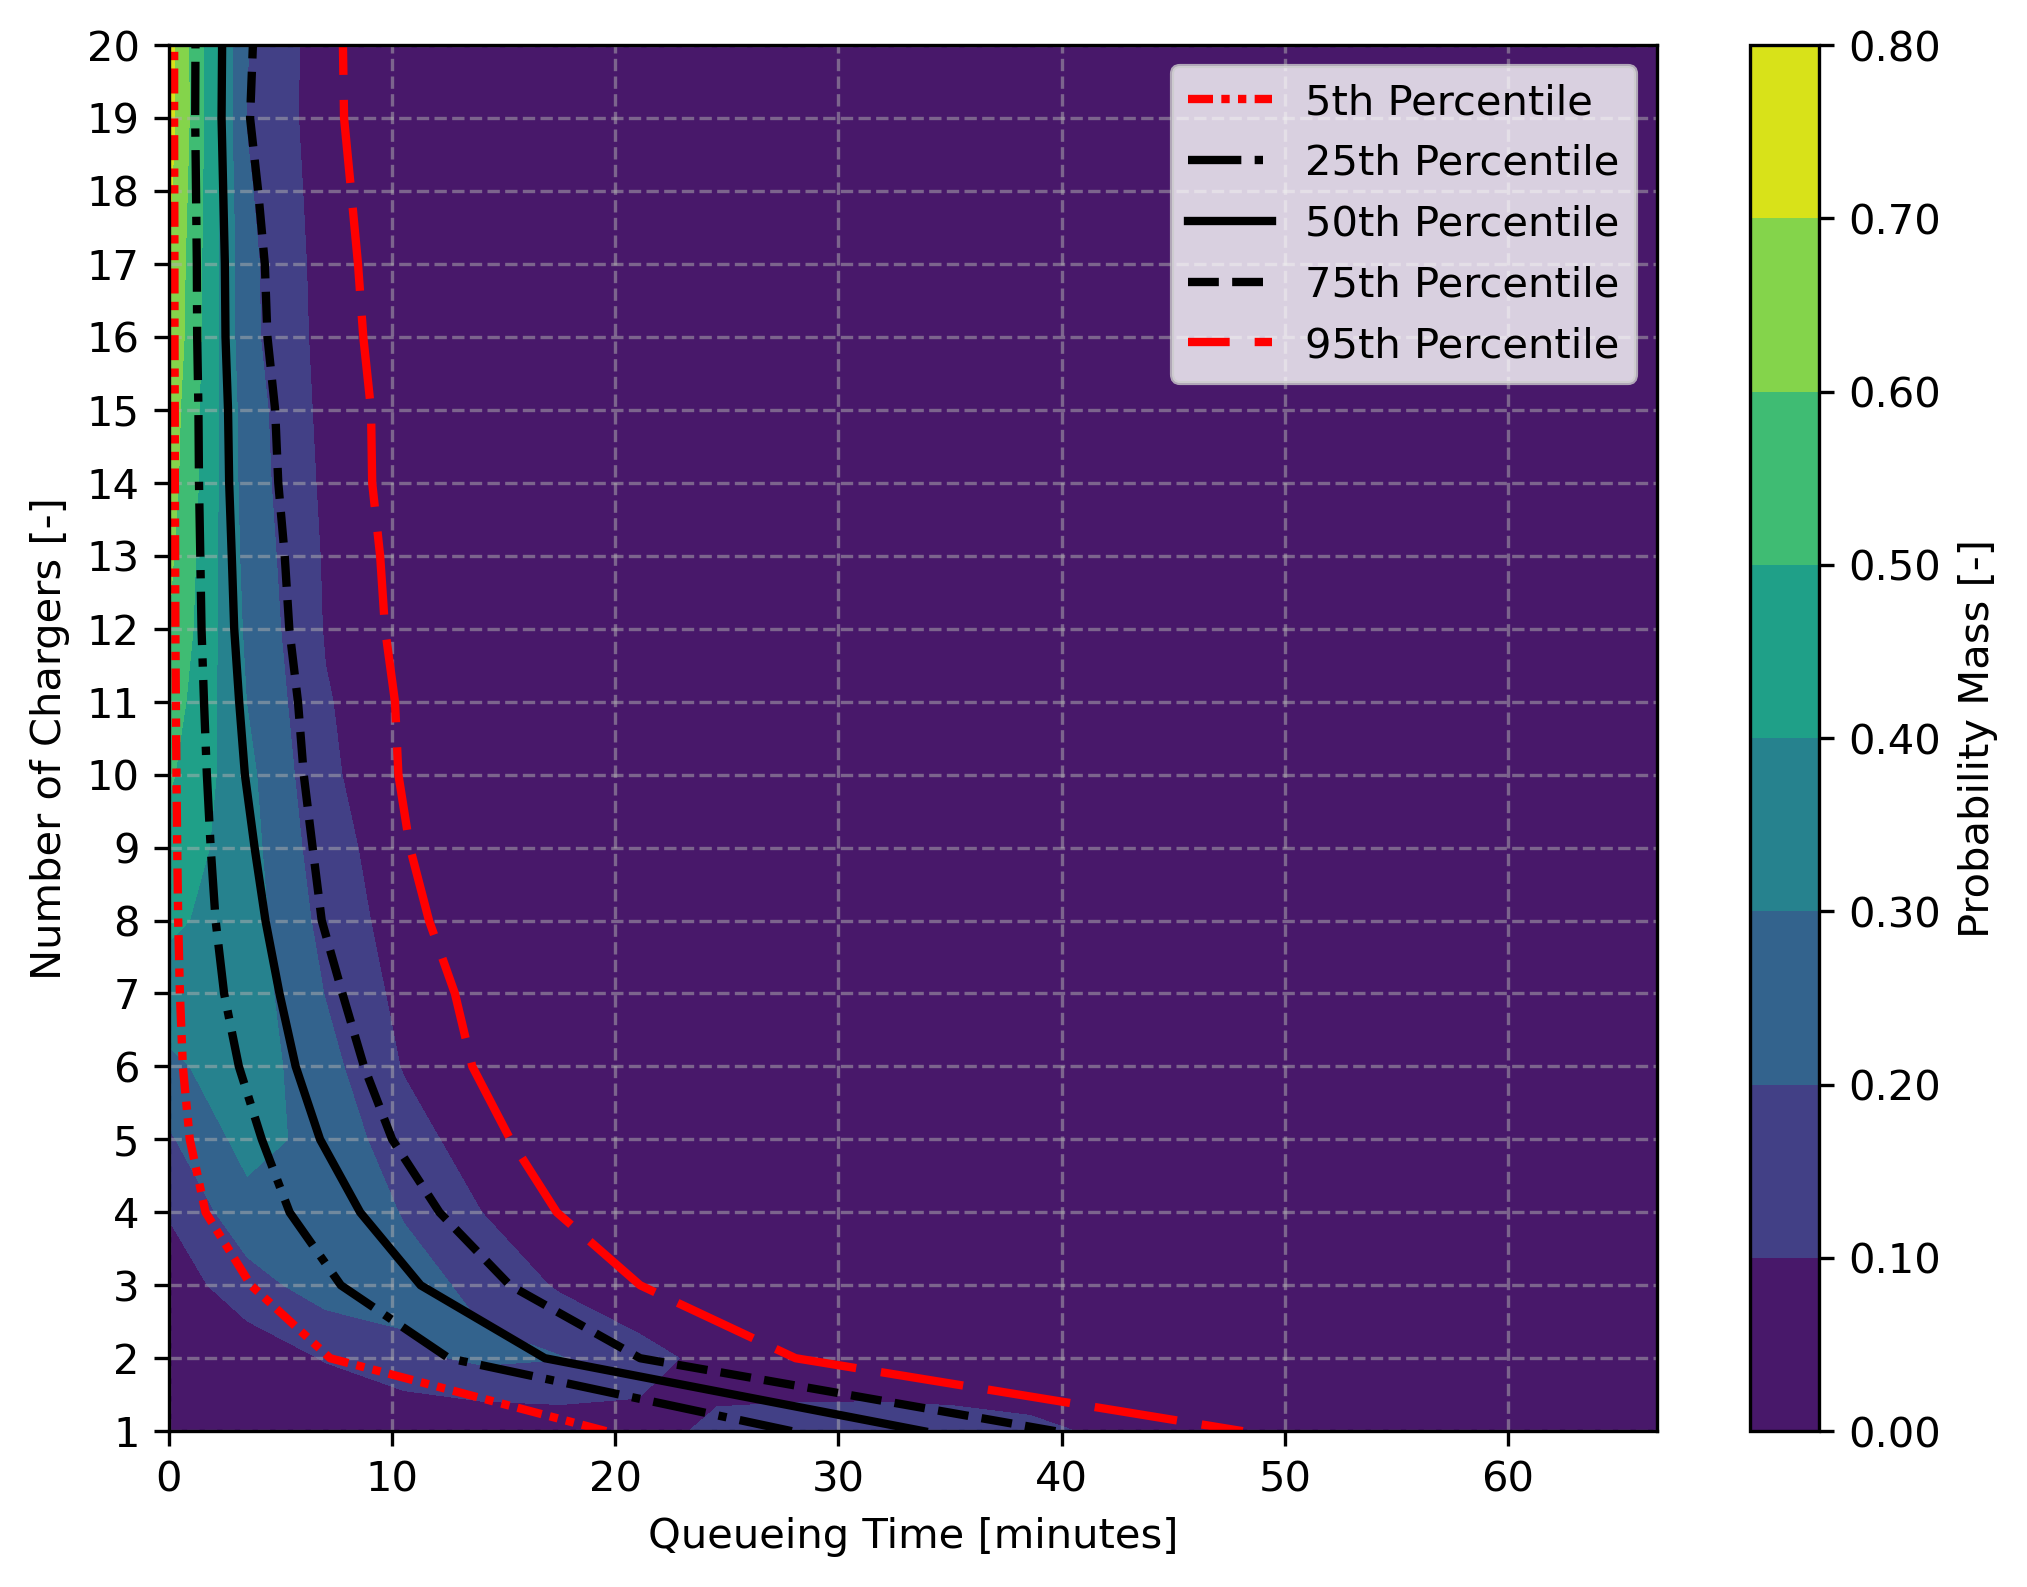
\includegraphics[width = \linewidth]{figs/expected_delay_contourf_1.png}
%	\caption{PDFs of expected delay time for station with mean arrival ratio of 1, constant mean charge energy delivered of 45 kWh, and different in-station redundancy.}
%	\label{fig:expected_delays_coutnours_1}
%\end{figure}
%
%\begin{figure}[H]
%	\centering
%	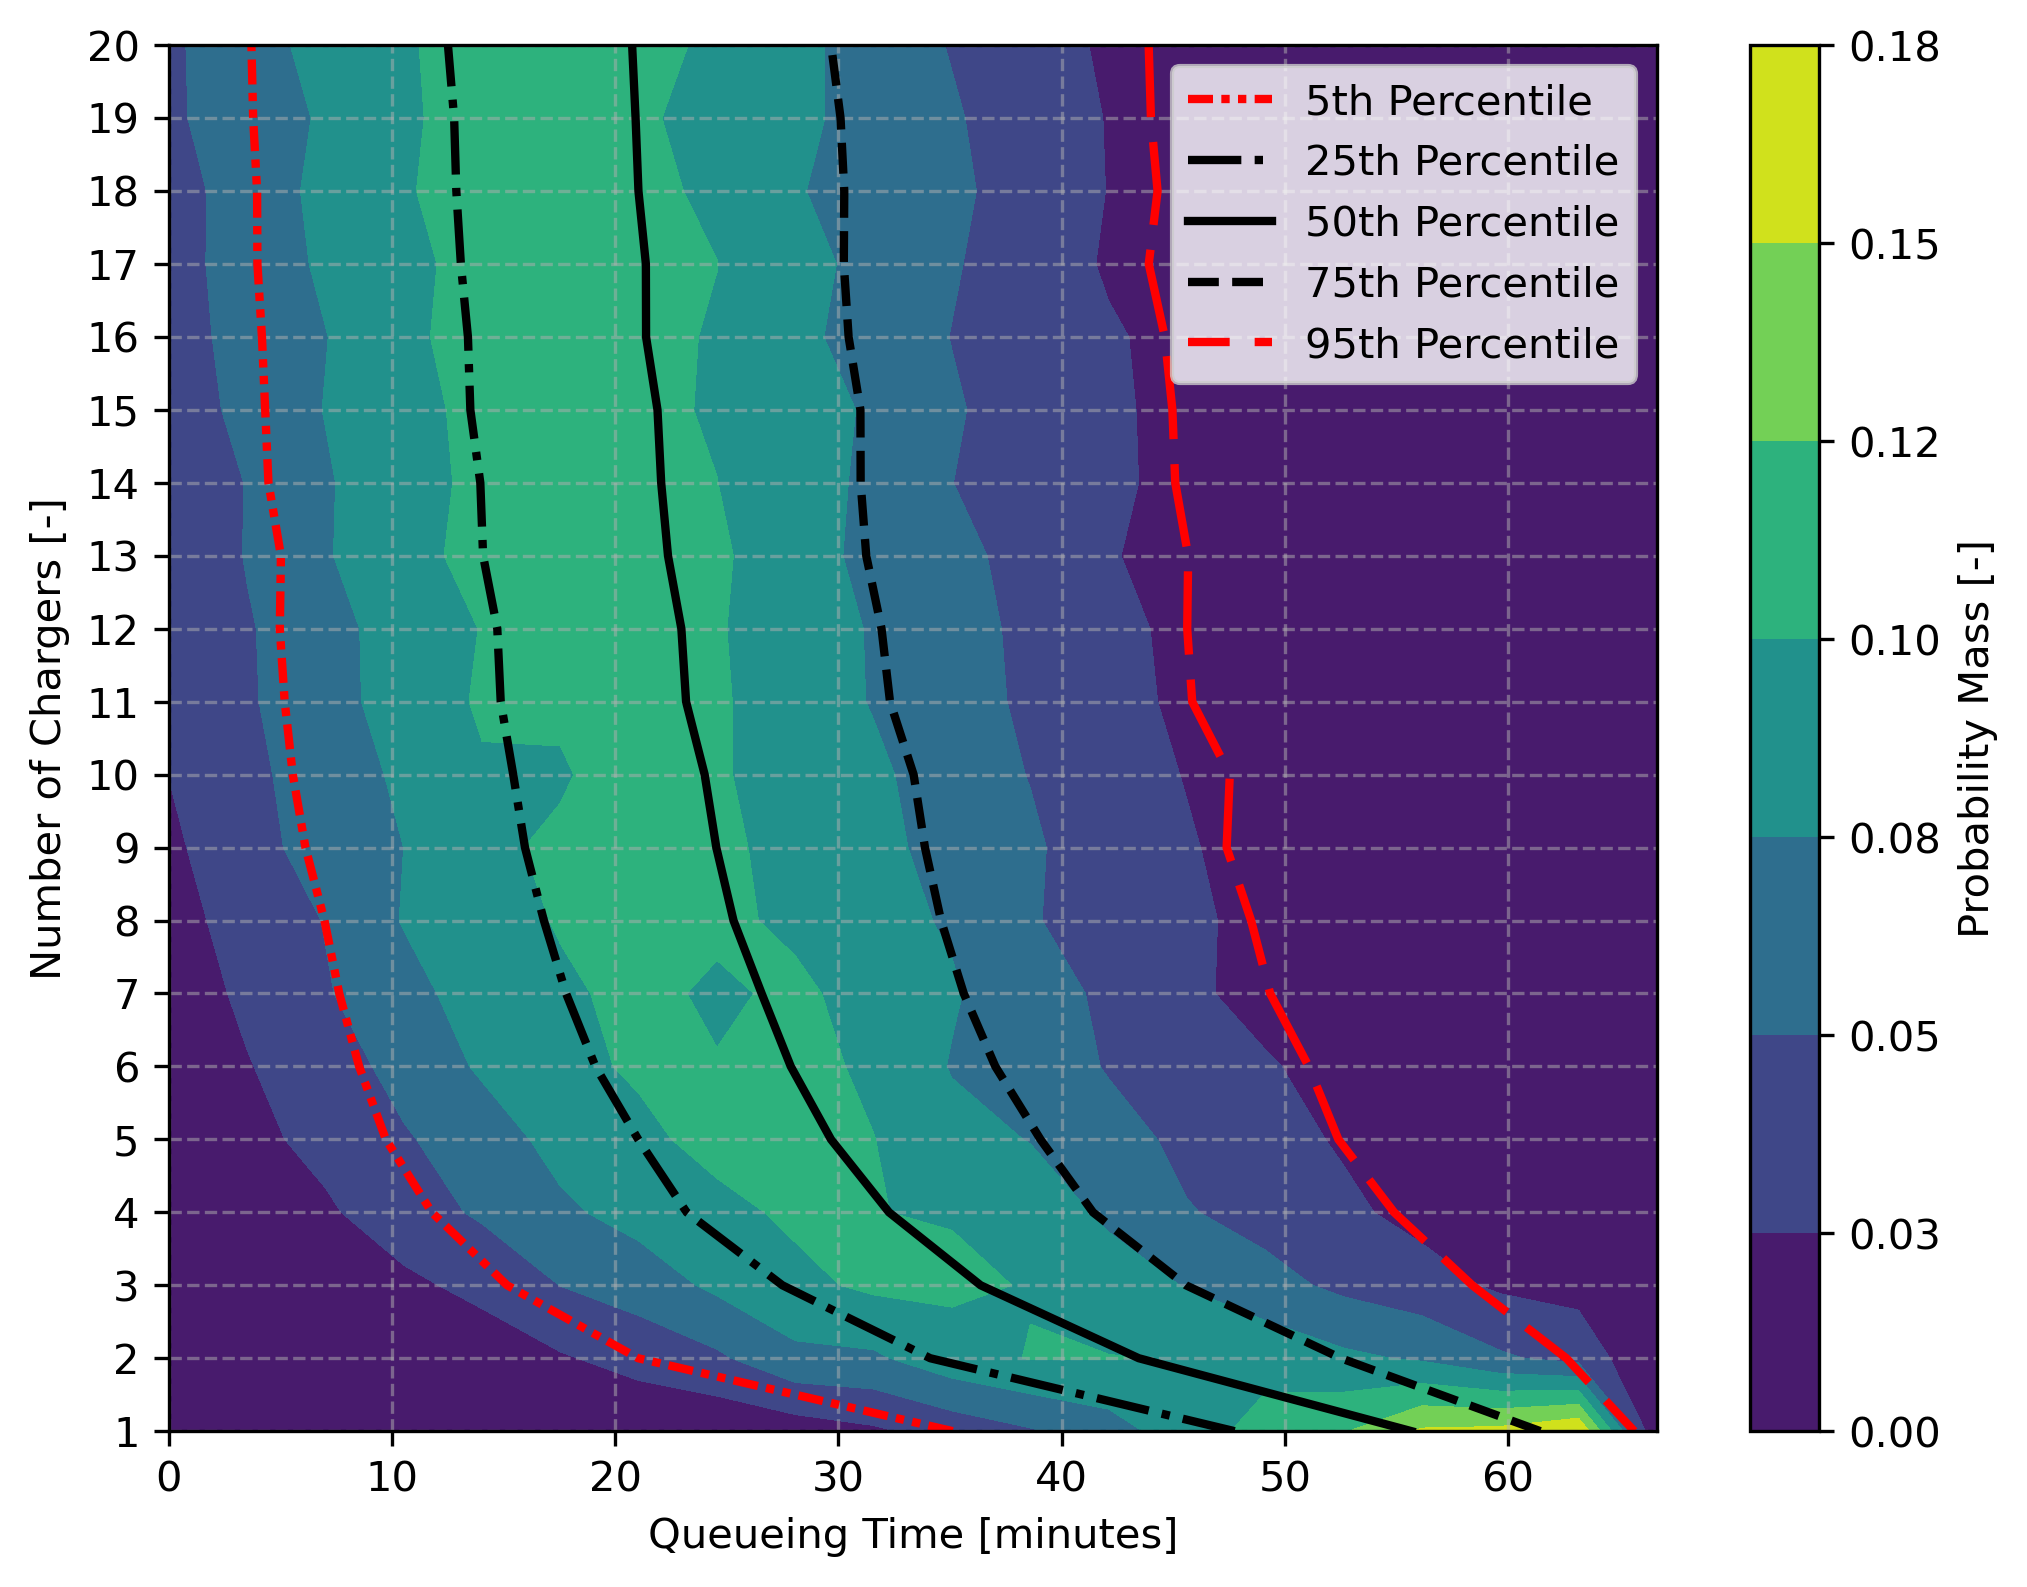
\includegraphics[width = \linewidth]{figs/expected_delay_contourf_2.png}
%	\caption{PDFs of expected delay time for station with mean arrival ratio of 2, constant mean charge energy delivered of 45 kWh, and different in-station redundancy.}
%	\label{fig:expected_delays_coutnours_2}
%\end{figure}
%
%\begin{figure}[H]
%	\centering
%	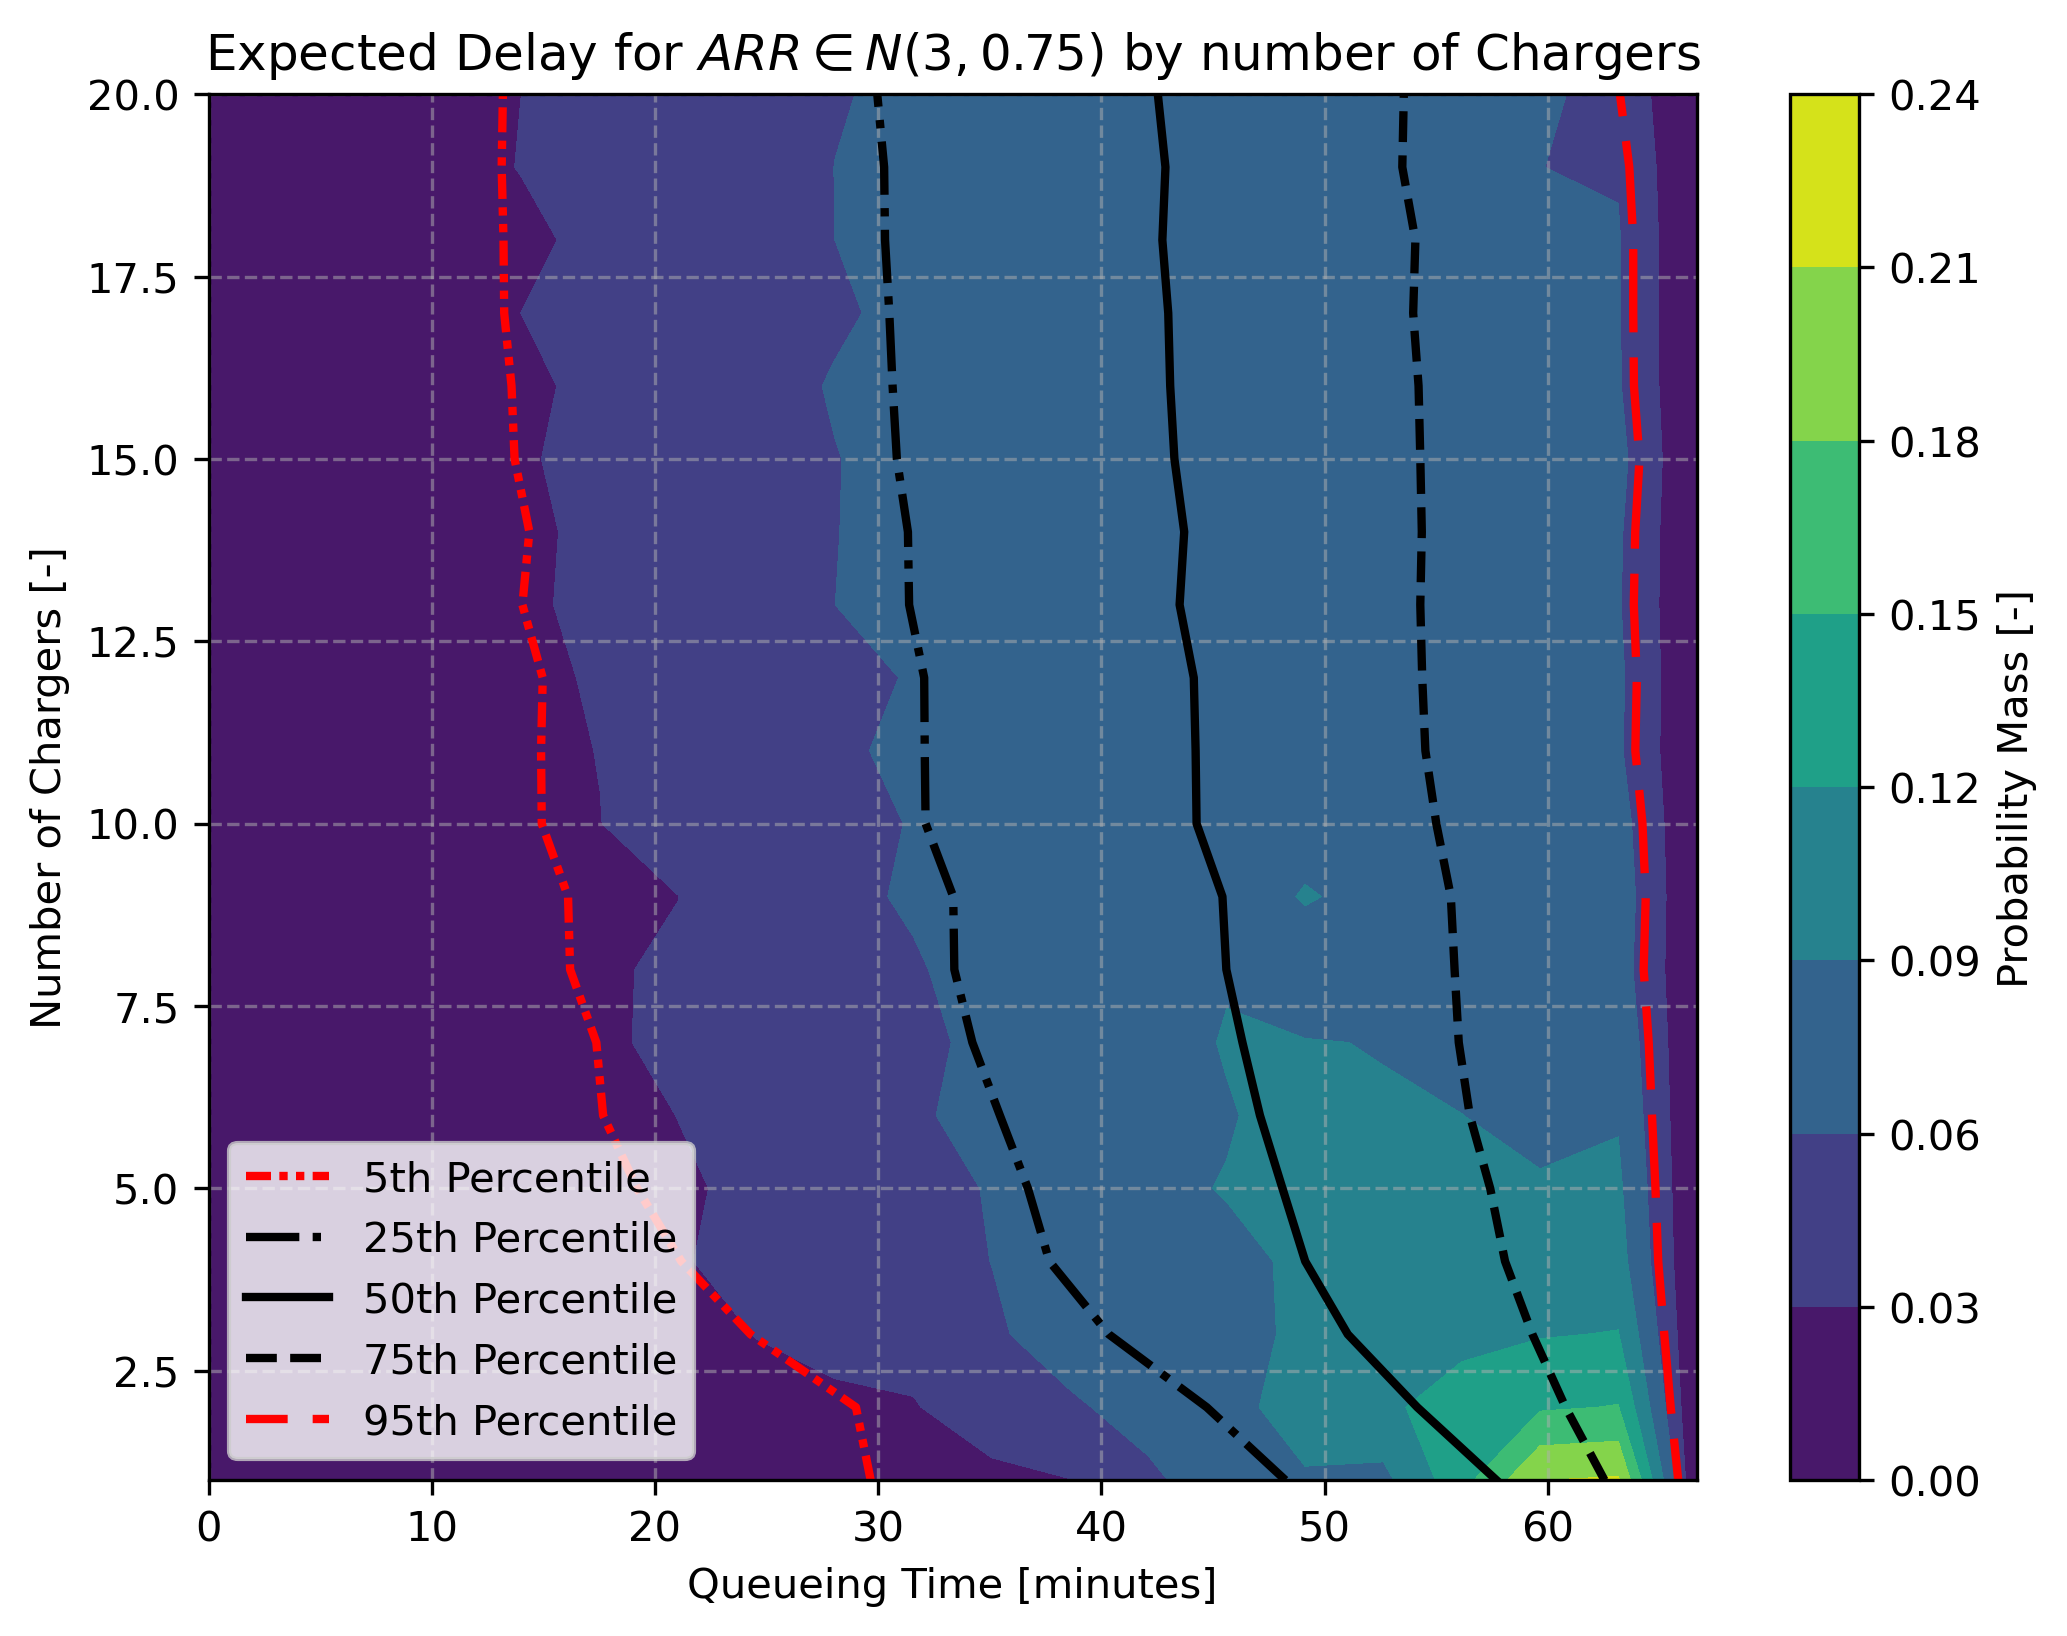
\includegraphics[width = \linewidth]{figs/expected_delay_contourf_3.png}
%	\caption{PDFs of expected delay time for station with mean arrival ratio of 3, constant mean charge energy delivered of 45 kWh, and different in-station redundancy.}
%	\label{fig:expected_delays_coutnours_3}
%\end{figure}